% Regression analysis o state estimation?
\section{Análisis de regresión}
\label{sec:regressionanalysis}
El análisis de regresión es un análisis estadístico para predecir el valor de una variable cuantitativa continua. Basándose en un conjunto de variables independientes, se busca estimar la relación de las mismas con una variable dependiente, mediante la obtención de una curva que mejor se ajuste a los datos disponibles, sin que necesariamente pase por todos ellos. En concreto, el modelo de regresión puede representarse como
\begin{equation}
    y_i = f(\bm{x}_i; \bm{\beta}) + v_i,
    \label{eq:regressionmodel}
\end{equation}
donde la variable $y_i$ corresponde a la respuesta o medición para el caso $i$, con $i = 1, 2, ..., m$, $\bm{x}_i = (x_{i1}, x_{i2}, ..., x_{in})$ corresponde al conjunto de valores, fijos o aleatorios, utilizados para explicar o predecir el comportamiento de $y_i$, conocidas como las \textit{variables regresivas} o \textit{independientes}, $\bm{\beta} = (\beta_1, \beta_2, ..., \beta_n)$ a los parámetros desconocidos\footnote{A diferencia de un estado, el que se define como una magnitud física que varía a través del tiempo, el parámetro es constante a través del tiempo.} a estimar, y $v_i$ a la componente de ruido propia para ese caso.

En base a esto, lo que se busca es estimar la función $f$ que mejor se ajuste a los datos, conocida como \textit{función de expectativa} para el modelo de regresión. Para ello, primero lo que debe hacerse es determinar la forma de dicha función que, en base a esta, se puede clasificar en \textit{regresión lineal} y \textit{regresión no lineal}.

Existen diferentes métodos dentro del análisis de regresión para poder estimar los parámetros desconocidos $\beta$, por lo que en las siguientes subsecciones se presentarán algunos de ellos, los cuales son de relevancia para el seguimiento de la tesis.

% En cambio, cuando la función que modela al sistema \textit{no puede expresarse como una combinación lineal de los parámetros desconocidos} $\bm{\beta}$, se trata entonces de una regresión no lineal, y debe realizarse un proceso iterativo para encontrar la curva que mejor se adapte al sistema.

% La información de tales relaciones se efectúa a partir de información muestral acerca de los valores tomados por $y$, $x_1$, $x_2$, $x_3$, ..., $x_n$, y trata de cuantificar la magnitud de la dependencia entre ellas.

\subsection{Regresión lineal}
En regresión lineal, la variable $y$ \textit{es una combinación lineal} de los parámetros, es decir,
\begin{align}
    y_i &= \beta_1 x_{i1} + \beta_2 x_{i2} + \beta_3 x_{i3} + ... + \beta_n x_{in} + v_i \\
      &= \bm{x}_i \bm{\beta} + v_i
\end{align}

\subsubsection{Método de cuadrados mínimos ordinario (OLS)}
Con el fin de hallar los parámetros desconocidos, uno de los métodos más utilizados corresponde al \textit{método de cuadrados mínimos}, el cual plantea que el valor más probable de dichos parámetros será aquel que minimiza la suma de los errores cuadráticos entre lo que se observa y lo que se espera. Este método es una variante especial del problema más general, en el que dada una función $f:\mathbb{R}^n\rightarrow\mathbb{R}$ se busca un argumento de $f$ que de el mínimo valor de la llamada \textit{función de coste}
\begin{equation}
    \hat{x} = argmin_x f(x)
    \label{eq:globalminimizer}
\end{equation}
llamado tambien como el \textit{minimzador global}.

Si se quiere, por ejemplo, medir el peso de una bolsa de naranjas, cuyo valor real es $x$, con el uso de una balanza de poca precisión, el valor medido $y$ puede modelarse como el valor real corrompido por ruido, $v$, linealmente mediante la ecuación
\begin{equation}
    y = x + v
    \label{eq:linearmeasmodel}
\end{equation}

Para cada una de las mediciones, se define un término escalar de ruido que es independiente de los otros términos de error ya que, para este caso, se asume que el ruido es independiente y de distribución uniforme. Ahora, si se define el error entre cada medición y el valor verdadero de la bolsa de naranjas, se obtiene el denominado \textit{criterio de error} de cada medición, esto es,
\begin{equation}
    e_i = y_i - x
\end{equation}

Con estos errores definidos, el método de cuadrados mínimos define que la mejor estimación del valor $x$ es la que minimiza el \textit{criterio de error cuadrático}
\begin{equation}
    \hat{x}_{OLS} = argmin_x(e_1^2+e_2^2+e_3^2+...+e_m^2) = \mathscr{L}_{OLS}(x),
    \label{eq:squarederrorcriterion}
\end{equation}

% Luego de un set de cinco mediciones realizadas por separado y en forma secuencial, se obtienen los valores que se observan en la Tabla \ref{tab:naranjasbalanza}, junto con sus modelos de medición y errores cuadráticos.

% \begin{table}[]
\centering
\begin{tabular}{c|c|c|c}
\textbf{Medición} & \textbf{Peso {[}g{]}} & \textbf{Modelo de medición} & \textbf{Error} \\ \hline
1                       & 1012                  & $y_1 = x + v_1$        & $e_1 = y_1 - x$      \\ \hline
2                       & 989                   & $y_2 = x + v_2$        & $e_2 = y_2 - x$      \\ \hline
3                       & 1008                  & $y_3 = x + v_3$        & $e_3 = y_3 - x$      \\ \hline
4                       & 1030                  & $y_4 = x + v_4$        & $e_4 = y_4 - x$      \\ \hline
5                       & 971                   & $y_5 = x + v_5$        & $e_5 = y_5 - x$           
\end{tabular}
\caption{Peso de una bolsa de naranjas para cada medición realizada}
\label{tab:naranjasbalanza}
\end{table}

Para poder minimizar la función de coste, suponiendo que fueron tomadas cinco mediciones realizadas por separado y en forma secuencial, primero hay que reescribir a la función de error en su forma matricial, siendo entonces
\begin{align}
    \bm{e} &= \bm{y} - \bm{H}\cdot x \\
    \begin{bmatrix}
        e_1\\ e_2\\ e_3\\ e_4\\ e_5
    \end{bmatrix}
    &= 
    \begin{bmatrix}
        y_1\\ y_2\\ y_3\\ y_4\\ y_5
    \end{bmatrix}
    -
    \begin{bmatrix}
        1\\ 1\\ 1\\ 1\\ 1
    \end{bmatrix}
    x
\end{align}
con $\bm{H}$ la \textit{matriz Jacobiana} que, para este caso particular, posee valores unitarios. Dicha matriz tiene las dimensiones de $m\times n$, donde \textit{m} es el número de mediciones y \textit{n} es el número de parámetros que se desean estimar. Por ello, \textit{x} si bien en este caso es un escalar, puede ser un vector en el caso que se tengan múltiples indeterminaciones. En base a esto, se puede redefinir a la función de coste como

\begin{align}
    \mathscr{L}_{OLS}(x) &= \bm{e}^T\bm{e} \\
                        &= (\bm{y} - \bm{H}x)^T(\bm{y} - \bm{H}x) \\
                        &= \bm{y}^T\bm{y} - x^T\bm{H}^T\bm{y} - \bm{y}^T\bm{H}x + x^T\bm{H}^T\bm{H}x
\end{align}

Para minimizar esta ecuación, se procede a computar la derivada parcial de la función de coste respecto a la incertidumbre $x$ para luego igualarla a cero.
\begin{align}
    \frac{\partial \mathscr{L}}{\partial x}\bigg\rvert_{x=\hat{x}} = -\bm{y}^T\bm{H} - \bm{y}^T\bm{H} + 2\hat{x}^T\bm{H}^T\bm{H} &= 0 \\
    -2\bm{y}^T\bm{H} + 2\hat{x}^T\bm{H}^T\bm{H} &= 0
\end{align}

Despejando, se llega al valor del peso de la bolsa de naranjas que minimiza el criterio de error cuadrático
\begin{equation}
    \hat{x}_{OLS} = (\bm{H}^T\bm{H})^{-1}\bm{H}^T\bm{y}
\end{equation}

Esta expresión tiene solución si y solo si existe $(\bm{H}^T\bm{H})^{-1}$, o sea, si la matriz tiene inversa. Si tenemos \textit{m} mediciones y \textit{n} parámetros,
\begin{align*}
    \bm{H} &\in \Re^{m\times n} \\
    \bm{H}^T\bm{H} &\in \Re^{n\times n}
\end{align*}

Por lo tanto, para que $(\bm{H}^T\bm{H})^{-1}$ exista es necesario que se dispongan mínimamente de la misma cantidad de mediciones que variables a estimar, esto es
\begin{equation*}
    m \geq n
\end{equation*}

\subsubsection{Método de cuadrados mínimos ponderado (WLS)}

Volviendo al ejemplo de la bolsa de naranjas, si se toman mediciones con distintas balanzas, es lógico pensar que mientras mayor sea la precisión de cada una, mayor importancia tendrá su valor indicado para determinar el peso de la bolsa. Si se considera al modelo de medición lineal con \textit{m} mediciones y \textit{n} incertidumbres,
\begin{align}
    \begin{bmatrix}
        y_1 \\ . \\ . \\ . \\ y_m
    \end{bmatrix}
    &=
    \bm{H}
    \begin{bmatrix}
        x_1 \\ . \\ . \\ . \\ x_n
    \end{bmatrix}
    +
    \begin{bmatrix}
        v_1 \\ .\\ . \\ . \\ v_m
    \end{bmatrix} \\
    \bm{y} &= \bm{H} \bm{x} + \bm{v}
\end{align}

En cuadrados mínimos ordinarios, se asume implícitamente que cada término de error, $v_i$, posee el mismo desvío estándar, $\sigma$. En cambio, si se toma que cada término de error es independiente pero con distinto desvío estándar,
\begin{equation}
    \mathbb{E}_{[v_i^2]} = \sigma_i^2 \hspace{0.5cm}(i=1,...,m)\hspace{1cm}\bm{R}=\mathbb{E}_{[\bm{v}\bm{v}^T]} = 
    \begin{bmatrix}
        \sigma_1^2  &        &     0      \\
                    & \ddots &            \\
            0       &        & \sigma_m^2
    \end{bmatrix}
\end{equation}
se puede definir a partir de esto el \textit{criterio de cuadrados mínimos ponderado} como
\begin{align}
    \mathscr{L}_{WLS}(x) &= \bm{e}^T\bm{R}^{-1}\bm{e} \\
                         &= \frac{e_1^2}{\sigma_1^2} + \frac{e_2^2}{\sigma_2^2} + ... + \frac{e_m^2}{\sigma_m^2}
\end{align}

Mientras mayor sea el ruido esperado, menor será el peso que tenga en la medición. En el caso que todos los desvíos sean iguales, \textit{no afecta el valor estimado final}, ya que pasa a ser una constante dividiendo a todos los errores.

Expandiendo el nuevo criterio,
\begin{align}
    \mathscr{L}_{WLS}(x) &= \bm{e}^T\bm{R}^{-1}\bm{e} \\
                         &= (\bm{y} - \bm{H}\bm{x})^T\bm{R}^{-1}(\bm{y}-\bm{H}\bm{x})
\end{align}

Como en el caso de los cuadrados mínimos ordinarios, la ecuación MONGO puede minimizarse realizando el gradiente en este caso al ser que se cuentan con \textit{n} incógnitas.
\begin{equation}
    \frac{\partial \mathscr{L}}{\partial \bm{x}}\bigg\rvert_{\bm{x}=\hat{\bm{x}}} = -\bm{y}^T\bm{R}^{-1}\bm{H} + \hat{\bm{x}}^T\bm{H}^T\bm{R}^{-1}\bm{H} = 0
\end{equation}

obteniendo entonces las ecuaciones normales ponderadas
\begin{equation}
    \hat{\bm{x}}_{WLS} = (\bm{H}^T\bm{R}^{-1}\bm{H})^{-1} \bm{H}^T\bm{R}^{-1}\bm{y}
\end{equation}

\subsubsection{Método de cuadrados mínimos recursivo (RLS)}

Hasta el momento, todos los datos de las mediciones se encontraban disponibles. Ahora, si lo que se tiene es, por ejemplo, un sensor que entrega datos cada cierto tiempo, con el razonamiento utilizado hasta el momento se tendería a pensar que es necesario correr alguno de los métodos vistos cada vez que llega un dato nuevo con todo el set completo. Se puede apreciar que claramente esto produciría un aumento de costo computacional a medida que transcurre el tiempo, haciendo que en un punto llegue a ser un problema.

Para evitar este problema, lo que se busca es un método recursivo que mantenga un estimador actual del parámetro óptimo para todas las mediciones que se han recolectado hasta ese momento, y luego actualizar dicho estimador dada la medición en el intervalo de tiempo actual. Para lograr esto, se puede utilizar entonces un \textit{estimador lineal recursivo}.

Suponiendo que se tiene un estimador óptimo $\hat{\bm{x}}_{k-1}$ de los parámetros desconocidos en el tiempo $k-1$ con ruido blanco Gaussiano aditivo, al llegar la nueva medición en el tiempo $k$,
\begin{equation}
    \bm{y}_k = \bm{H}_k \bm{x} + \bm{v}_k
\end{equation}

Por lo tanto, el objetivo es poder computar $\hat{\bm{x}}_k$ como una función de $\bm{y}_k$ y $\hat{\bm{x}}_{k-1}$.

Un estimador lineal recursivo está dado por
\begin{equation}
    \hat{\bm{x}}_k = \hat{\bm{x}}_{k-1} + \bm{K}_k (\bm{y}_k - \bm{H}_k \hat{\bm{x}}_{k-1})
\end{equation}
donde $\bm{K}_k$ es una matriz de ganancia del estimador, el término entre paréntesis se denomina la innovación, y cuantifica que tan bien la medición actual se equipara con el mejor estimador previo. Aún sin conocer la matriz $\bm{K}_k$, en dicha ecuación puede observarse que el nuevo estimador es la suma del estimador anterior y el término correctivo basado en la diferencia entre lo esperado de la medición y lo que acutalmente se midió. Si la innovación fuese igual a cero, se mantendría el estimador anterior.

Finalmente, para el término $\bm{K}_k$, lo que se busca es minimizar el \textit{valor esperado de la suma de errores cuadráticos} del estimador actual en el tiempo \textit{k}. Para un solo parámetro escalar,
\begin{align}
    \mathscr{L}_{RLS}(x) &= \mathbb{E}_{[(x_k - \hat{x}_k)^2]} \\
                         &= \sigma_k^2
\end{align}

En cambio, si se tienen \textit{n} parámetros desconocidos en el tiempo \textit{k}
\begin{align}
    \mathscr{L}_{RLS}(x) &= \mathbb{E}_{[(x_{1k} - \hat{x}_{1k})^2 + ... + (x_{nk} - \hat{x}_{nk})^2]} \\
                         &= tr(\bm{P}_k)
\end{align}

siendo $tr()$ la \textit{traza} (o \textit{trace})\footnote{Corresponde a la suma de los elementos de la diagonal principal de la matriz} de la matriz de covarianza $\bm{P}_k$. En lugar de minimizar directamente el error, lo que se minimiza es su valor esperado, el cual es la varianza del estimador. A menor varianza, mayor será el grado de confianza del estimador.

Al igual que antes, es posible expresar a la covarianza en función de $\bm{K}_k$ utilizando la formulación lineal recursiva
\begin{equation}
    \bm{P}_k = (\bm{1} - \bm{K}_k\bm{H}_k)\bm{P}_{k-1}(\bm{1}-\bm{K}_k\bm{H}_k)^T + \bm{K}_k\bm{R}_k\bm{K}_k^T
\end{equation}

Mediante el uso de cálculo matricial y derivadas parciales, se puede llegar a que este término se minimiza cuando
\begin{equation}
    \bm{K}_k = \bm{P}_{k-1}\bm{H}_k^T(\bm{H}_k\bm{P}_{k-1}\bm{H}_k^T + \bm{R}_k)^{-1}
\end{equation}

En base a esto, es posible reescribir la ecuación de la matriz de covarianza como
\begin{align}
    \bm{P}_k &= \bm{P}_{k-1} - \bm{K}_k\bm{H}_k\bm{P}_{k-1} \\
                 &= (\bm{1} - \bm{K}_k\bm{H}_k)\bm{P}_{k-1}
\end{align}

De este último término se puede observar que cuanto más grande sea la matriz de ganancia $\bm{K}$, será más pequeña la nueva covarianza del estimador. Por lo tanto, se puede decir que la covarianza \textit{se encoge} con cada medición.

Resumiendo, el algoritmo de los cuadrados mínimos recursivos consta de tres pasos
\begin{enumerate}
    \item Inicializar los parámetros desconocidos y la matriz de covarianza. Esta predicción inicial, por ejemplo, puede obtenerse a partir de la primer medición que se toma y la covarianza puede venir de especificaciones técnicas.
        \begin{align}
            \hat{\bm{x}}_0 &= \mathbb{E}_{[\bm{x}]} \\
            \bm{P}_0 &= \mathbb{E}_{[(\bm{x} - \hat{\bm{x}}_0)(\bm{x} - \hat{\bm{x}}_0)^T]}
        \end{align}
    \item Definir el Jacobiano y la matriz de covarianza de la medición
        \begin{equation}
          \bm{y}_k = \bm{H}_k\bm{x}+\bm{v}_k
        \end{equation}
    \item Actualizar el valor estimado de $\hat{\bm{x}}_k$ y la covarianza $\bm{P}_k$
        \begin{align}
            \bm{K}_k &= \bm{P}_{k-1}\bm{H}_k^T(\bm{H}_k\bm{P}_{k-1}\bm{H}_k^T + \bm{R}_k)^{-1} \\
            \hat{\bm{x}}_k &= \hat{\bm{x}}_{k-1} + \bm{K}_k(\bm{y}_k - \bm{H}_k\hat{\bm{x}}_{k-1}) \\
            \bm{P}_k &= (\bm{1} - \bm{K}_k\bm{H}_k)\bm{P}_{k-1}
        \end{align}
\end{enumerate}

\subsubsection{Método de máxima verosimilitud (MLE)}

En lugar de escribir una pérdida tal como se realiza en cuadrados mínimos, puede aproximarse el problema de la estimación de parámetros óptimos al buscar qué parámetros hacen que las mediciones obtenidas sean las más probables. En otras palabras, cuál \textit{x} maximiza la probabilidad condicional de $\bm{y}$
\begin{equation}
    \hat{x} = argmax_x p(\bm{y}|x)
    \label{eq:maxlikelihood}
\end{equation}

Volviendo al ejemplo de la bolsa de naranjas, si se tienen cuatro posibles valores de dicho peso, como se observa en la Figura \ref{fig:mostlikelyproba}, el valor que maximiza la verosimilitud condicional dada la medición $y_{med}$ corresponde a $x_b$, ya que es la densidad de probabilidad mayor en la ubicación medida.
\begin{figure}[!h]
    \centering
    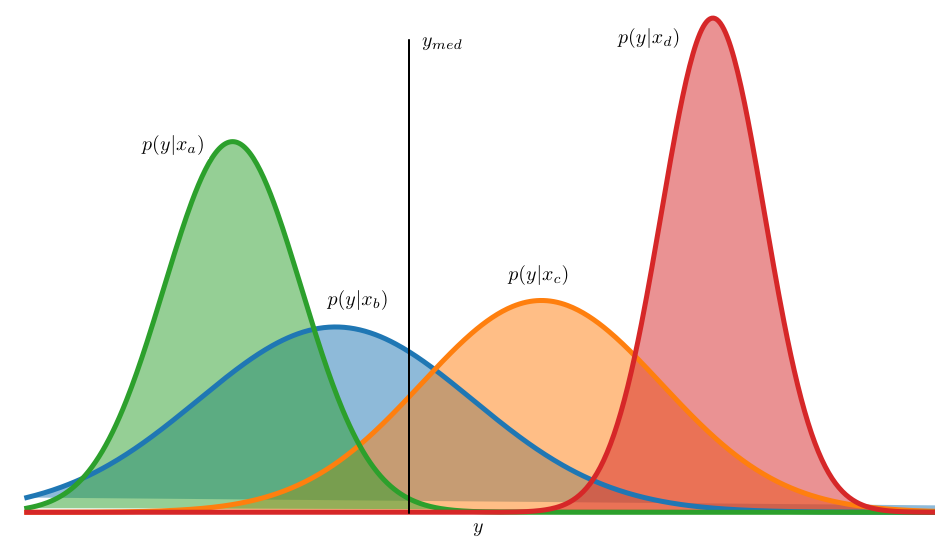
\includegraphics[width=\textwidth]{Img/MostLikelyProba.png}
    \caption{Posibles valores del peso de la bolsa de naranjas y su valor real $y_{med}$}
    \label{fig:mostlikelyproba}
\end{figure}

Tomando en cuenta el modelo de medición presente en la Ecuación (\ref{eq:linearmeasmodel}), el mismo puede ser expresado como una probabilidad condicional de la medición, asumiendo alguna densidad de probabilidad para $v$, por ejemplo, ruido blanco Gaussiano aditivo
\begin{equation}
    v \sim \mathcal{N}(0,\sigma^2)
\end{equation}
entonces, el parámetro desconocido, $x$, resulta ser la media de esta densidad, y la varianza corresponde a la varianza de ruido.
\begin{equation}
    p(y|x) = \mathcal{N}(x,\sigma^2)
\end{equation}

Teniendo en cuenta que la función densidad de probabilidad de una Gaussiana es
\begin{equation}
    \mathcal{N}(z;\mu,\sigma^2) = \frac{1}{\sigma \sqrt{2\pi}} e^{\frac{-(z-\mu)^2}{2\sigma^2}}
\end{equation}

puede expresarse la medición de verosimilitud para una de las mediciones como
\begin{align}
    p(y|x) &= \mathscr{N}(y;x,\sigma^2) \\
           &= \frac{1}{\sqrt{2\pi\sigma^2}} e^{\frac{-(y-x)^2}{2\sigma^2}}
\end{align}

Si se tienen múltiples mediciones independientes, entonces
\begin{align}
    p(\bm{y}|x) &\propto \mathscr{N}(y_1;x,\sigma^2)\cdot\mathscr{N}(y_2;x,\sigma^2)\cdot...\cdot\mathscr{N}(y_m;x,\sigma^2) \\
            &= \frac{1}{\sqrt{(2\pi)^m\sigma^{2m}}} \exp\left({\frac{-\sum_{i=1}^m(y_i-x)^2}{2\sigma^2}}\right)
\end{align}
y el estimador de máxima verosimilitud (MLE) será
\begin{equation}
    \hat{x}_{MLE} = argmax_x p(\bm{y}|x)
\end{equation}

En lugar de tratar de optimizar el verosímil directamente, puede aplicarse el logaritmo
\begin{align}
    \hat{x}_{MLE} = argmax_x \log p(\bm{y}|x)
    \label{eq:mlewithlog}
\end{align}
y, como la función logaritmo aumenta monotónicamente
\begin{equation}
    \log p(\bm{y}|x) = -\frac{1}{2\sigma^2}\left((y_1-x)^2+...+(y_m-x)^2\right)+C
\end{equation}

Esta expresión es similar a la suma de los errores cuadráticos, presentada en (\ref{eq:squarederrorcriterion}). La constante $C$ en esta expresión refiere a términos que no son funciones de $x$ y pueden ser ignorados.

Luego, como el argumento que maximiza la función $f$ es equivalente al negativo del argumento que minimiza dicha función, o sea,
\begin{equation}
    argmax_z f(z) = argmin_z \left(-f(z)\right)
\end{equation}
el problema de la máxima verosimilitud puede ser escrito como
\begin{align}
    \hat{x}_{MLE} &= argmin_x -\left(\log p(\bm{y}|x)\right) \\
                  &= argmin_x \frac{1}{2\sigma^2}\left((y_1-x)^2+...+(y_m-x)^2\right)
\end{align}

Por lo tanto, es posible realizar la maximización de la verosimilitud mediante una minimización de la suma de errores cuadráticos. Esto es válido ya que se asume que las mediciones se encuentran corrompidas por ruido blanco Gaussiano independiente aditivo de igual varianza.

Finalmente, si se asume que cada medición tiene una varianza distinta, se llega al mismo criterio que en cuadrados mínimos ponderados
\begin{equation}
    \hat{x}_{MLE} = argmin_x \frac{1}{2}\left(\frac{(y_1-x)^2}{\sigma_1^2}+...+\frac{(y_m-x)^2}{\sigma_m^2}\right) =\frac{1}{2} \bm{e}^T\bm{R}^{-1}\bm{e}
    \label{eq:mlewls}
\end{equation}

Resumiendo, en ambos casos, el estimador de máxima verosimilitud para ruido blanco Gaussiano es equivalente a las soluciones de los cuadrados mínimos ordinarios o ponderados.
\begin{equation}
    \hat{x}_{MLE} = \hat{x}_{OLS} = argmin_x\mathscr{L}_{OLS}(x) = argmin_x\mathscr{L}_{MLE}(x)
\end{equation}

Esto cobra importancia en sistemas realistas, los cuales presentan una gran cantidad de fuentes de ruido. Recordando el teorema central del límite, que establece que cuando se suman variables aleatorias independientes, su suma normalizada tenderá a una distribución normal, y teniendo en cuenta que el método de cuadrados mínimos es equivalente a calcular la máxima verosimilitud\footnote{Siempre asumiendo que se está en presencia de ruido blanco Gaussiano aditivo}, es posible calcular el mejor estimador de una forma computacionalmente sencilla.

Sin embargo, una consideración importante a tener en cuenta con el método de cuadrados mínimos es cuando se presenta un valor atípico, esto es, los que se encuentran en las ''colas'' de la Gaussiana, provocando que el estimador final se aleje del valor verdadero. Por ello es importante cuantificar la distribución de error antes de aplicar ciegamente máxima verosimilitud o cuadrados mínimos.

\subsubsection{Método de máximo a posteriori (MAP)}
En lugar de buscar las mediciones más probables como en el método de máxima verosimilitud, puede buscarse el \textit{posterior}, el cual está asociado a la probabilidad condicional que es asignada luego de tomar en cuenta la medición, esto es, $p(x|\bm{y})$. Mediante el uso de la regla de Bayes, el posterior puede expresarse como
\begin{align}
    p(x|\bm{y}) &= \frac{p(\bm{y}|x)p(x)}{p(\bm{y})} 
    \label{eq:posteriorfull}\\
    &\propto p(\bm{y}|x)p(x)
    \label{eq:posterior}
\end{align}

Reemplazando en la Expresión (\ref{eq:maxlikelihood}) por el posterior, entonces
\begin{align}
    \hat{x}_{MAP} &= argmax_x\ p(\bm{y}|x)p(x) \\
                  &= argmax_x\ \log p(\bm{y}|x) + \log p(x)
\end{align}
se obtiene la \textit{expresión del máximo a posteriori}. A diferencia del método de máxima verosimilitud, en el máximo a posteriori se incluye a la probabilidad previa (o \textit{prior}) $p(x)$. Lo que significa es que, la probabilidad ahora está ponderada con algo de peso proveniente del prior.

Puede entonces decirse que el método de máxima verosimilitud es un caso especial del máximo a posteriori, donde la probabilidad prior es uniforme.

\subsection{Regresión no lineal}

La regresión lineal es un método muy utilizado para analizar los datos descriptos por modelos que son lineales en los parámetros. Sin embargo, muchas veces las formas de las curvas que mejor ajustan a los datos obtenidos son no lineales en los parámetros. En estos casos, el modelo de regresión sigue siendo de la misma forma que el de la Expresión (\ref{eq:regressionmodel}), a diferencia de que al menos una de las derivadas de la función de expectativa con respecto a los parámetros depende de al menos uno de los parámetros\footnote{Por ejemplo, si derivo $\theta_1 \theta_2 x_1$ respecto a cualquiera de esos dos parámetros, dicha derivada parcial dependerá del parámetro no derivado}.

Para diferenciar entre modelos lineales y no lineales, los parámetros para este último caso se definen con $\bm{\theta}$,
\begin{equation}
    y_i = f(\bm{x}_i, \bm{\theta}) + v_i
    \label{eq:nonlinearregressionmodel}
\end{equation}

El criterio de error cuadrático para modelos no lineales es uno general, del cual puede derivarse la Expresión (\ref{eq:squarederrorcriterion})
\begin{align}
    \mathscr{S}(\bm{\theta}) &= \sum_{i=1}^n (y_i - f(\bm{x}_i;\bm{\theta}))^2 \\
                   &= (\bm{y} - \bm{f}(\bm{\theta}))^T\bm{R}^{-1}(\bm{y} - \bm{f}(\bm{\theta})) \\
                   &= \bm{y}^T \bm{R}^{-1}\bm{y} - 2\bm{y}^T\bm{R}^{-1}\bm{f}(\bm{\theta}) + \bm{f}(\bm{\theta})^T\bm{R}^{-1}\bm{f}(\bm{\theta})
    \label{eq:generalsquarederrorcriterion}
\end{align}
donde $\bm{f}(\bm{\theta}) = (f_1(\bm{\theta}), f_2(\bm{\theta}), ..., f_n(\bm{\theta}))$ y $f_i(\bm{\theta}) = f(\bm{x}_i;\bm{\theta})$.

A diferencia de la situación de cuadrados mínimos lineales, $\mathscr{S}(\bm{\theta})$ puede tener varios mínimos relativos además del mínimo absoluto $\hat{\bm{\theta}}$. Por ello, si bien el \textit{minimizador global} presentado en la Expresión (\ref{eq:globalminimizer}) es válido para este tipo de modelos, este problema es muy difícil de resolver en general, por lo que se presentan sólo métodos para resolver el problema más simple de encontrar un minimizador local para $f$, un vector de argumento que proporciona un valor mínimo de $f$ dentro de una determinada región cuyo tamaño está dado por $\gamma$, donde $\gamma$ es pequeño y positivo. Entonces, debe cumplirse que

\begin{equation}
    f(\theta^*) \leq f(\theta)\hspace{1cm}\text{para}\hspace{1cm}||\theta - \theta^*|| < \gamma
    \label{eq:localminimizer}
\end{equation}
conocido como el \textit{minimizador local}.

La minimización de $\mathscr{S}$ respecto a sus parámetros debe ser realizada iterativamente.
%El objetivo de cada iteración es encontrar una perturbación $\bm{\delta}$ a los parámetros $\bm{\theta}$ que reduzca $\mathscr{S}$.
Desde un punto inicial $\bm{\theta}_0$, el método produce una serie de vectores $\bm{\theta}_1$, $\bm{\theta}_2$, ..., los cuales se espera que converjan a $\bm{\theta}^*$, un minimizador local para la función dada. La mayoría de los métodos tienen medidas que imponen la \textit{condición descendente}
\begin{equation}
    \bm{f}_{i+1}(\bm{\theta}) < \bm{f}_{i}(\bm{\theta})
    \label{eq:descendingcondition}
\end{equation}

Esto evita la convergencia a un maximizador y también hace menos probable que se converja hacia un punto de silla\footnote{Punto sobre una superficie en el que la pendiente es cero pero no se trata de un extremo local, sino que la elevación es máxima en una dirección y mínima en la dirección perpendicular.}. Si la función dada tiene varios minimizadores, el resultado dependerá del punto de partida $\bm{\theta}_0$. No se sabe a priori cuál de los minimizadores se encontrarán, por lo que no es necesariamente el minimizador más cercano a $\bm{\theta}_0$.

En muchos casos, el método produce vectores que convergen hacia el minimizador en dos etapas claramente diferentes. Cuando $\bm{\theta}_0$ está lejos de la solución, se busca que el método produzca iteraciones que se muevan constantemente hacia $\bm{\theta}^*$. En esta ''etapa global'' de la iteración, es necesario que los errores no aumenten, excepto en los primeros pasos, es decir
\begin{equation}
    ||\bm{e}_{k+1}|| < ||\bm{e}_k||\hspace{1cm}\text{para}\hspace{1cm}k<K
\end{equation}
donde $\bm{e}_k$ responde a la función de error
\begin{equation}
    \bm{e}_k = \bm{\theta}_k - \bm{\theta}^*
\end{equation}

En la etapa final de la iteración, donde $\bm{\theta}_k$ es cercano a $\bm{\theta}^*$, se quiere una convergencia más rápida. A partir de esto pueden distinguirse tres casos
\begin{itemize}
    \item \textit{Convergencia lineal}
    \begin{equation}
            ||\bm{e}_{k+1}|| \leq a||\bm{e}_k||\hspace{1cm}\text{cuando $||e_k||$ es pequeño}\hspace{1cm}0<a<1
    \end{equation}
    \item \textit{Convergencia cuadrática}
    \begin{equation}
        ||\bm{e}_{k+1}||=O(||\bm{e}_k||^2)\hspace{1cm}\text{cuando $||\bm{e}_k||$ es pequeño}
    \end{equation}
    \item \textit{Convergencia superlineal}
    \begin{equation}
        \frac{||\bm{e}_{k+1}||}{||\bm{e}_k||}\rightarrow 0\hspace{1cm}\text{para $k\rightarrow 0$}
    \end{equation}
\end{itemize}

Estos métodos presentados son \textit{métodos de descenso} que satisfacen la condición descendiente de la Expresión (\ref{eq:descendingcondition}) en cada paso de la iteración. Un paso del iterador actual consiste en
\begin{itemize}
    \item Encontrar una \textit{dirección de descenso} $\bm{\delta}_d$, el cual lo será para $\bm{f}$ en $\bm{\theta}$ si $\bm{\delta}^T\bm{f}'(\bm{\theta}) < 0$. En caso de no existir $\bm{\delta}$, entonces $\bm{f}'(\bm{\theta}) = 0$, representando en este caso que $\bm{\theta}$ es estacionario.
    \item Si existe $\bm{\delta}$, hallar una longitud de paso que de una buena disminución en el valor $\bm{f}$ en la dirección dada por $\bm{\delta}_d$, con tal de obtener una disminución en el valor de la función objetivo.
\end{itemize}

Una forma de hacer esto mediante el proceso llamado \textit{búsqueda de línea}, el cual consiste en hallar una aproximación a
\begin{equation}
    \alpha_e = argmin_{\alpha > 0} \bm{f}(\bm{\theta}+\alpha \bm{\delta})
\end{equation}

\subsubsection{Método de descenso de gradiente}

El método de descenso de gradiente es un método de minimización general que actualiza los valores de los parámetros en la dirección de descenso más pronunciada, esto es, la dirección opuesta al gradiente de la función objetivo. La idea detrás de este método radica en moverse repetidamente en la dirección del gradiente negativo (llamado el \textit{descenso más pronunciado}) hasta que converja. El método de descenso de gradiente converge bien para problemas con funciones objetivas simples. Para problemas con muchos parámetros, este método es a veces la única opción viable.

Volviendo al caso de la Expresión (\ref{eq:generalsquarederrorcriterion}), el gradiente de dicha función con respecto a los parámetros es
\begin{align}
    \frac{\partial \mathscr{S}}{\partial \bm{\theta}}\bigg\rvert_{\bm{\theta}=\hat{\bm{\theta}}} &= 2(\bm{y} - \bm{f}(\hat{\bm{\theta}}))^T \bm{R}^{-1}\frac{\partial}{\partial \bm{\theta}}(\bm{y} - \bm{f}(\hat{\bm{\theta}}) \\
    &= -2(\bm{y} - \bm{f}(\hat{\bm{\theta}}))^T \bm{R}^{-1}\left[\frac{\partial \bm{f}(\hat{\bm{\theta}})}{\partial \hat{\bm{\theta}}}\right] \\
    &= -2(\bm{y} - \bm{f}(\hat{\bm{\theta}}))^T \bm{R}^{-1}\bm{J}
\end{align}
donde la \textit{matriz Jacobiana} $\bm{J}$ representa la sensibilidad local de la función $\bm{f}$ a variaciones de los parámetros $\hat{\bm{\theta}}$\footnote{Intuitivamente, la matriz Jacobiana indica qué tan rápido está cambiando cada salida de la función a lo largo de cada dimensión de entrada}. Tener en cuenta que en los modelos que son lineales en los parámetros, $\bm{f} = \bm{X}\bm{\theta}$, el Jacobiano es la matriz de los vectores base del modelo, $\bm{X}$. La actualización de parámetros $\bm{\delta}$ que mueve los parámetros en la dirección del descenso más pronunciado viene dada por
\begin{equation}
    \bm{\delta}_{gd} = \alpha\bm{J}^T\bm{R}^{-1}(\bm{y} - \bm{f}(\hat{\bm{\theta}}))
\end{equation}
donde el escalar positivo $\alpha$ determina la longitud del escalón en la dirección de descenso más pronunciada.

\subsubsection{Método de Gauss-Newton}
El método de Gauss-Newton es un método para minimizar una función objetivo de suma de cuadrados. Presume que la función objetivo es aproximadamente cuadrática en los parámetros cercanos a la solución óptima. Para problemas de tamaño moderado, el método de Gauss-Newton generalmente converge mucho más rápido que el método de descenso de gradiente.

La función evaluada con parámetros de modelo perturbados puede aproximarse localmente a través de una expansión de la serie Taylor de primer orden.
\begin{equation}
    \bm{f}(\hat{\bm{\theta}+\bm{\delta}}) \approx \bm{f}(\hat{\bm{\theta}}) + \left[\frac{\partial \bm{f}}{\partial \hat{\bm{\theta}}}\right]\bm{\delta} = \bm{f}(\hat{\bm{\theta}}) + \bm{J}\bm{\delta}
    \label{eq:gaussnewtontaylor}
\end{equation}

Substituyendo la Expresión (\ref{eq:gaussnewtontaylor}) en (\ref{eq:generalsquarederrorcriterion}) para $\mathscr{S}(\bm{\theta} + \bm{\delta})$
\begin{equation}
    \begin{aligned}
        \mathscr{S}(\bm{\theta}+\bm{\delta}) \approx{} &\bm{y}^T\bm{R}^{-1}\bm{y} + \bm{f}(\bm{\theta})^T\bm{R}^{-1}\bm{f}(\bm{\theta}) - 2\bm{y}^T\bm{R}^{-1}\bm{f}(\bm{\theta}) - \\
        & -2\left(\bm{y} - \bm{f}(\bm{\theta})\right)^T\bm{R}^{-1}\bm{J}\bm{\delta} + \bm{\delta}^T\bm{J}^T\bm{R}^{-1}\bm{J}\bm{\delta}
    \end{aligned}
\end{equation}
La aproximación de Taylor de primer orden  de la Expresión (\ref{eq:gaussnewtontaylor}) da como resultado una aproximación para $\mathscr{S}$ que es cuadrática en $\bm{\delta}$. Por lo tanto, el $\bm{\delta}$ que minimiza a $\mathscr{S}$ se encuentra cuando $\frac{\partial \mathscr{S}}{\partial \bm{\delta}} = 0$
\begin{equation}
    \frac{\partial}{\partial \bm{\delta}}\mathscr{S}(\bm{\theta} + \bm{\delta}) \approx -2\left(\bm{y} - \bm{f}(\bm{\theta})\right)^T\bm{R}^{-1}\bm{J} + 2\bm{\delta}^T\bm{J}^T\bm{R}^{-1}\bm{J}
\end{equation}
y las ecuaciones normales resultantes para la actualización de Gauss-Newton son
\begin{equation}
    \left[\bm{J}^T\bm{R}^{-1}\bm{J}\right]\bm{\delta}_{gn} = \bm{J}^T\bm{R}^{-1}(\bm{y} - \bm{f}(\bm{\theta})
\end{equation}

\subsubsection{Método de Levenberg-Marquardt}
Aunque el Método de Gauss-Newton converge muy rápido cuando ya está cerca de la solución, puede fallar en dar un paso de descenso válido cuando el optimizador aún está lejos del mínimo buscado.

El algoritmo de Levenberg-Marquardt aborda este problema variando adaptativamente las actualizaciones de parámetros entre la actualización de descenso de gradiente y la actualización de Gauss-Newton,
\begin{equation}
    \left[\bm{J}^T\bm{R}^{-1}\bm{J} + \lambda\bm{I}\right]\bm{\delta}_{lm} = \bm{J}^T\bm{R}^{-1}\left(\bm{y} - \bm{f}(\bm{\theta}\right)
\end{equation}{}
donde pequeños valores del \textit{parámetro de amortiguación} $\lambda$ resultan en una actualización de Gauss-Newton, mientras que valores grandes de $\lambda$ llevan a una actualización de descenso de gradiente. El parámetro de amortiguación $\lambda$ se inicializa para que sea grande, de modo que las primeras actualizaciones sean pequeños pasos en la dirección de descenso más pronunciada. Si alguna iteración resulta en una peor aproximación $(\mathscr{S}(\bm{\theta} + \bm{\delta}_{lm}) > \mathscr{S}({\bm{\theta}}))$, entonces $\lambda$ aumenta. De lo contrario, a medida que la solución mejora, $\lambda$ disminuye, haciendo que el método de Levenberg-Marquardt se aproxima al método de Gauss-Newton, y la solución generalmente se acelera al mínimo local.

En la relación de actualización de Marquardt
\begin{equation}
    \left[\bm{J}^T\bm{R}^{-1}\bm{J} + \lambda\;  diag(\bm{J}^T\bm{R}^{-1}\bm{J})\right]\bm{\delta}_{lm} = \bm{J}^T\bm{R}^{-1}\left(\bm{y} - \bm{f}(\bm{\theta})\right)
\end{equation}{}
los valores de $\lambda$ se normalizan a los valores de $\bm{J}^T\bm{R}^{-1}\bm{J}$.

En sistemas donde solo hay un mínimo, el método de Levenberg-Marquardt convergerá al mínimo global incluso si la suposición inicial es arbitraria. En cambio, en sistemas con mínimos múltiples, es más probable que el método encuentre el mínimo global si la suposición inicial se encuentra próxima a la solución. Sin embargo, el mismo permite que la selección de valores iniciales esté más lejos de la solución que el método de Gauss-Newton.

Si bien existen numerosas implementaciones de este método, se presentará a continuación la solución propuesta por la \textit{librería Eigen}.
